\documentclass[12pt]{article}
\usepackage{amsmath}
\usepackage{amssymb}
\usepackage{graphicx}
\usepackage{hyperref}

% indent the first paragraph after section headings
\usepackage{indentfirst}

% Use natbib + BibTeX (avoids biblatex/logreq issues)
\usepackage{natbib}
\bibliographystyle{apalike}  % you can change to plainnat etc.

\title{Final Project \\ \vspace{0.5em} David Munson}

\begin{document}
	
	\maketitle
	
	\section{Introduction}
	
	\indent The goal of this project is to model the supply of trucks in the U.S. domestic trucking market. I aim to characterize the conditions under which firms are willing to add trucks to their fleets and to estimate the spot freight rate at which firms can expect to break even. The trucking industry is well known for its pronounced cyclicality: when market conditions are favorable firms expand capacity by acquiring tractors and in downturns they reduce fleet size or exit altogether. These decisions are inherently dynamic, forward-looking, and shaped by agents’ expectations about future profitability. I will attempt to formalize this behavior through a dynamic programming framework in which firms choose fleet size to maximize discounted profits.
	
	\indent A key insight that supports the structure of my model is that spot freight rates reflect the marginal cost of the least expensive truck available for hire. Shippers purchasing transportation services on the spot market typically regard carriers as homogeneous as long as they satisfy DOT regulations and maintain the required insurance and safety certifications. At the margin driver skill, equipment type, and carrier identity are not able to command higher prices, making the spot market a relatively undifferentiated segment of the industry.
	
	While many trucking firms do obtain more profitable long-term contracts through specialized services, the option to deploy an additional truck into the spot market remains available to nearly all carriers. Hence, any firm considering expansion weighs the cost of adding a truck against the expected profitability of operating that truck in the spot market.
	
	The first step of the project is to build a model of an individual firm or owner-operator deciding whether to enter the market and determining its optimal fleet size over time. This model will serve as the foundation for a broader market-level equilibrium analysis. The key difference to extrapolate this model to a further market equilibrium would be to make the stochastic spot rate be endogenously determined by the economy wide fleet size and to add a gradual drift upwards as the economy and population grows. In future work the model can be calibrated using data from the Department of Transportation and allow us to recover the underlying cost structure of trucking firms and to estimate the break-even spot price under which capacity will be added or reduced. The industry context and empirical patterns we rely on are discussed in practitioners' coverage (e.g., FreightWaves) and the academic literature \citep{freightwaves2025,harris2023long,miller2018arima}.
	
	\section{Single Firm Model}
	
	\subsection{Parameters}
	
	\indent The state consists of the firm's current fleet size $K\in\{0,\dots,K_{\max}\}$ and the current spot-market freight rate $r>0$. We set $K_{\max}=10$, reflecting the fact that most new entrants begin as single-truck owner-operators and expand cautiously. Once the threshold of ten trucks is reached, firms generally experience changes in their fixed-cost structure that lie outside the scope of this model. The spot rate evolves endogenously according to a stochastic process described below. The firm chooses next period’s fleet size $K'\in\{0,\dots,K_{\max}\}$, with the additional restriction that expansion is limited to at most one truck per period ($K' \le K+1$).
	
	\indent We work in thousands of dollars per period for all monetary quantities and revenue/expenses on yearly estimates. The models key insights though are able to be interpreted in a monthly or even continuous fashion as these parameters scale accordingly. The calibrated parameters used in the model are:
	
	\begin{itemize}
		\item $O = 160$: operating cost per truck per period.  This constitutes a realistic estimate of driver pay (80), maintenance (25), fuel (45), insurance (20), and other expenses incurred (10).
		\item $\delta = 0.10$: depreciation rate per period reflecting average truck lifespan of 10 years / 1,000,000 miles.
		\item $F = 25$: fixed cost incurred only when the firm expands ($K'>K$), reflecting transaction costs and onboarding expenses.  CDL courses cost slightly more on average, but these smaller firms typically onboard drivers who already received training from larger companies or have paid the upfront cost of their CDL training independently.
		\item $r$: spot rate, measured in thousands of dollars per truck per year. The unconditional mean is set to $\bar r = 190$ reflecting a typical per mile spot rate of 1.90 * 100,000 miles.
		\item $P_{\text{base}} = 180$: per-unit truck price when $r=\bar r$.  This is an accurate estimate of a "sleeper-cab" truck over the last year while the market has been roughly in equilibrium. The effective truck price is state-dependent:
		\[
		P(r) = P_{\text{base}} \cdot \frac{r}{\bar r}.
		\]
		\item $\beta = 0.96$: is our discount factor.
	\end{itemize}
	
	\subsection{Spot-rate shocks}
	
	\indent Spot freight rates are highly correlated with the previous period. We assume the spot freight rate follows a stationary AR(1) process in logs:
	\begin{equation}
		\log r' = \mu + \rho\big(\log r - \mu\big) + \varepsilon',
		\qquad \varepsilon' \sim \mathcal{N}(0,\sigma_r^2),
	\end{equation}
	with $|\rho|<1$ ensuring stationarity. Let $P(r' \mid r)$ represent the transition function. This AR(1) characterization is standard in the forecasting literature for truckload spot rates (see \citealt{miller2018arima}) and is consistent with recent empirical work on relationships between contract and spot markets in trucking \citep{harris2023long}.
	
	\subsection{Flow payoff and adjustment terms}
	
	\indent The state-dependent truck price is:
	\[
	P(r) = P_{\text{base}} \cdot \frac{r}{\bar r}.
	\]
	
	We view truck prices as a function of existing spot rates as both new and used trucks sell for higher values during times where spot rates are high and at low values when the freight market is in a state of oversupply.
	
	Depreciation cost per period for a fleet of size $K$ is therefore:
	\[
	\text{Dep}(K,r) = \delta \, P(r)\, K.
	\]
	
	\indent The per-period operating profit when the firm operates $K$ trucks at spot rate $r$ is:
	\[
	\pi(K,r) 
	= K \cdot r 
	- K \cdot O
	- \delta P(r) K,
	\]
	
	Adjustment-related transactions from choosing next-period fleet size $K'$ are:
	
	\[
	\text{BuyCost}(K,K',r) 
	= \big(P(r) + F\big)\cdot \mathbf{1}\{K'=K+1\},
	\]
	
	\[
	\text{SaleProceeds}(K,K',r) 
	= P(r)\cdot (K-K')_+.
	\]
	
	Putting these together, the immediate payoff from choosing $K'$ in state $(K,r)$ is:
	\[
	\Pi(K,K',r)
	=
	\pi(K,r)
	- \big(P(r)+F\big)\cdot \mathbf{1}\{K'=K+1\}
	+ P(r)\,(K-K')_+.
	\]
	
	The firm may expand by at most one truck per period and may sell any number of trucks.
	
	\subsection{Bellman equation}
	
	\indent Let $V(K,r)$ denote the value function. The Bellman equation is:
	\begin{equation}
		\label{eq:bellman_stochastic}
		V(K,r)
		=
		\max_{K' \in \{0,\dots,K_{\max}\}}
		\Big\{
		\Pi(K,K',r)
		+ \beta \,
		\mathbb{E}\!\left[
		V(K',r')
		\,\middle|\,
		r
		\right]
		\Big\},
	\end{equation}
	where the expectation is taken with respect to the AR(1) transition $P(r' \mid r)$.
	
	\bibliography{refs}
	
	\section{Results}
	
	\subsection{Policy Function}
	
	The first figure I would like to reference is our policy heatmap.  Figure \ref{fig:policy} plots the fleet-adjustment rule $K'(K,z)$ as a function of the current fleet size $K$ and the spot-rate shock index discretized over the grid of possible rates $z$.
	 
	Our firms act as expected - expanding when a particular high value threshold is met while quickly downsizing fleets when our spot rate is at the low end of our range (low z = low spot rate r).  This is exciting as in my personal experience many firms exhibit this behavior in real life.  During downturns they will have 1 or 2 core drivers who keep the business in operation and when in boom they will hire family members, friends and basically anyone who has a CDL to capitalize on high rates.  This trend was especially notable during the pandemic when freight rates spiked significantly.
	
	I was a little surprised by how well our model approximated this behavior as we did not have any specific "firm entry" cost or barriers like credit availability - authority generation - or setup costs associated with a new firm entering but our model still approximated the behavior well.
	
	
	\begin{figure}[h!]
		\centering
		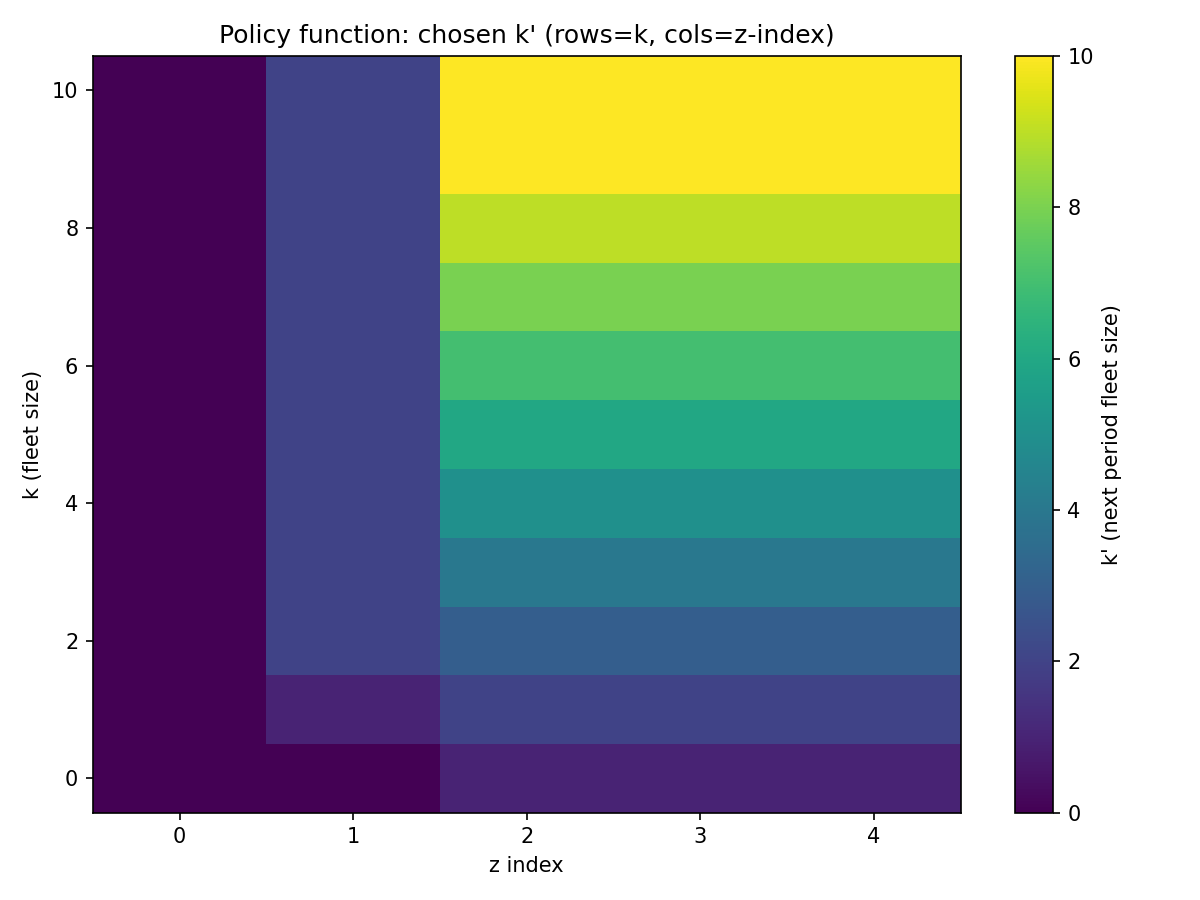
\includegraphics[width=0.8\textwidth]{results/figures/policy_heatmap.png}
		\caption{Optimal policy function $K'(K,z)$ across fleet sizes and spot-rate shock states.}
		\label{fig:policy}
	\end{figure}
	
	\subsection{Simulated Fleet Dynamics}
	
	We simulate the firm's behavior for 200 periods under the optimal policy. 
	The resulting time path of fleet size, shown in Figure \ref{fig:sim_ts}, reflects the cyclical investment behavior implied by the model. 
	When spot rates are persistently strong, the fleet grows toward the cap of 10 when adverse shocks occur capacity shrinks, sometimes very rapidly. 
	
	Another exciting result from our model is that firms tend to stay at lows and highs due to the persistence of our shocks.  This again mirrors the freight markets where large boom / bust periods typically go on for multiple years.

	\begin{figure}[h!]
		\centering
		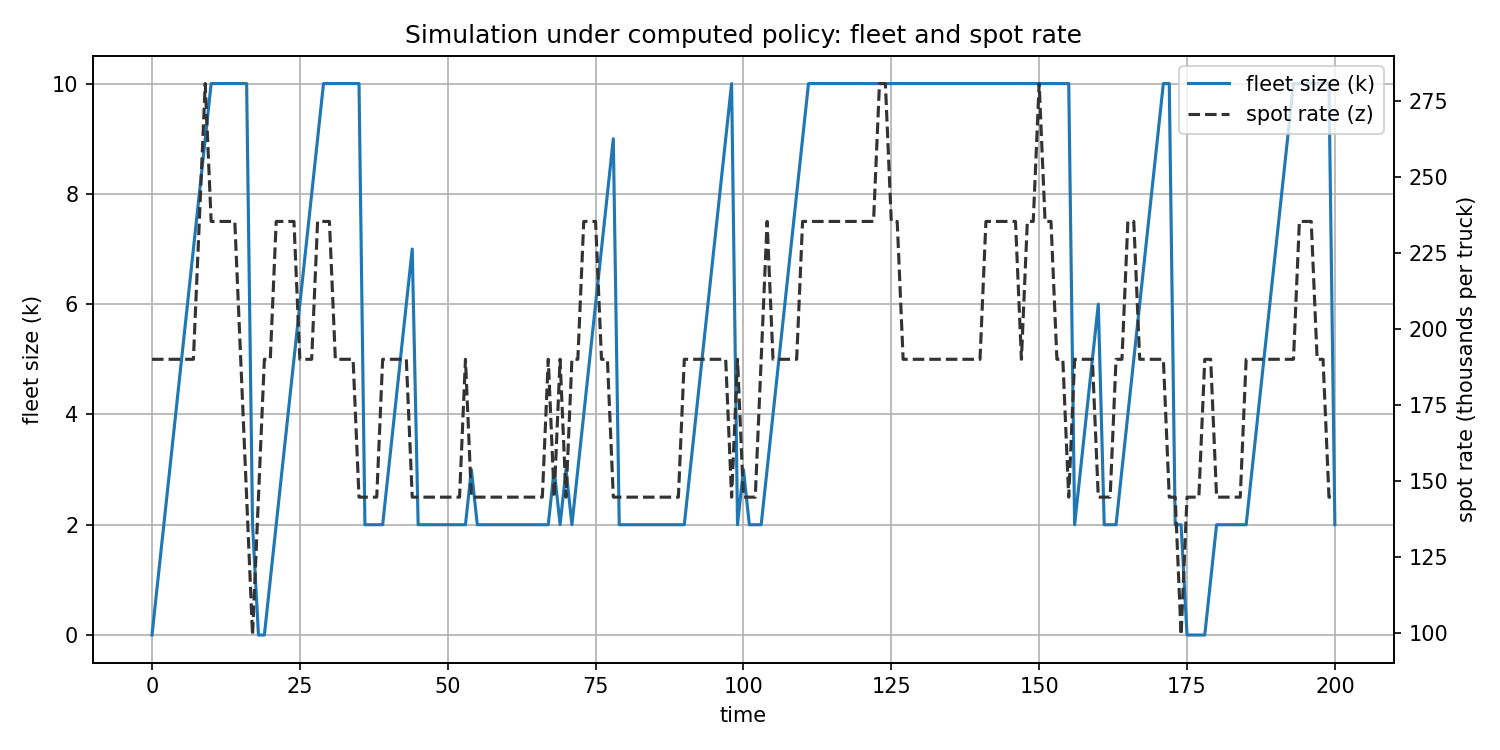
\includegraphics[width=0.95\textwidth]{results/figures/sim_timeseries.png}
		\caption{Simulated fleet size and spot-rate path over 200 periods.}
		\label{fig:sim_ts}
	\end{figure}
	
	\begin{figure}[h!]
		\centering
		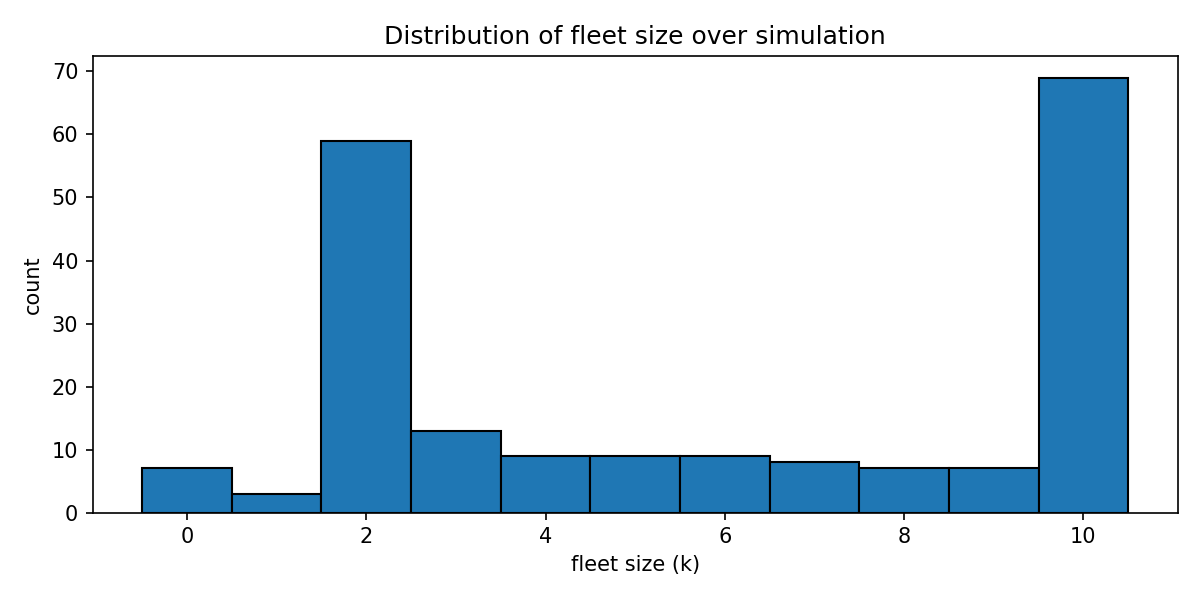
\includegraphics[width=0.9\textwidth]{results/figures/sim_histogram.png}
		\caption{Histogram of simulated fleet size distribution over time.}
		\label{fig:sim_hist}
	\end{figure}
	
	\subsection{Quantitative Summary}
	
	Table \ref{tab:summary} reports key statistics for the simulated economy. 
	The mean and median fleet sizes are 6.26 and 6.00 respectively, indicating a typical operator size between five and seven trucks. 
	Standard deviation is (3.36) which is consistent with the boom bust nature of this market.  
	Mean profit per period is approximately 102 (in thousands) which is again a very promising sign as that is a realistic figure for a typical small firm owner, The model also implies an average return on capital of 32.6\% which may seem high but that number is also capturing the labor that an owner puts into his business as well.  This is a key point as people in the trucking industry are largely indifferent between different professions and many of the small entrepreneurs are choosing trucking because it pays slightly higher than many similar small blue collar businesses.
	
	Periods with fleet size zero occur also only 3.5\% of the time, suggesting that complete exit is unlikely except during extended downturns.
	
	\begin{table}[h!]
		\centering
		\begin{tabular}{l c}
			\hline
			Statistic & Value \\ \hline
			Mean fleet size & 6.26 \\
			Median fleet size & 6.00 \\
			Standard deviation of fleet size & 3.36 \\
			Mean profit per period (thousands) & 101.55 \\
			Mean revenue per period (thousands) & 1183.95 \\
			Mean return on capital & 0.326 \\
			Percent of periods at $K=0$ & 3.5\% \\
			\hline
		\end{tabular}
		\caption{Simulation summary statistics.}
		\label{tab:summary}
	\end{table}
	
	\subsection{Economic Interpretation}
	
	Several economic mechanisms drive the results:
	
	\section{Conclusion}
	
	I am very pleased by the results of our dynamic programming model.  The policy function and empirical measures match industry numbers and decision making even with our rough guesses on parameters.  My next step to extend this model would be to build  
	
	One of the key challenge in parameterize this model is that data on profitability of these smaller firms is scarce and hard to discern. Many small business owners have unique arrangements with their power units and drivers and I don't believe the majority of small firms could generate a consistent estimation of profitability even if they were incentivized to.  Given models of medium and large companies we could begin to match our data to DOT data that tracks firm entry, exit and existing power units in operation with the end goal of finding a true measure of break-even rates and profitability.
	
	
\end{document}
